\documentclass[a4paper,11pt]{article}
\usepackage[T1]{fontenc}
\usepackage[utf8]{inputenc}
\usepackage{lmodern}
\usepackage{amssymb}
\usepackage{color}
\usepackage{graphicx}
\newcommand{\tab}{\hspace*{2em}}

\title{TI1805 Project: Raytracer}
\author{Better Late Than Never:\\
		Piet van Agtmaal 4321278\\
		Gerlof Fokkema <nr>\\
		Jente Hidskes 4335732\\
		Owen Huang <4317459>\\
		Arjan Langerak <nr>\\
		Skip Lentz <4334051>\\
		Dennis van Velzen <nr>\\
	   }

\begin{document}

\maketitle
Ray tracing does indeed deliver beautiful images. That is, if it supports enough graphics techniques. We think that our ray tracer delivers beautiful images and, before showing you the proof, we would like to give you a quick list of graphics techniques we have implemented:
\begin{itemize}
	\item Shading (Phong illumination model);
	\item Reflections;
	\item Refractions (inluding Schlick's approximation);
	\item Shadows;
	\item Textures;
	\item Anti-aliasing (jittered super-sampling);
	\item Hierarchical bounding box tree;
\end{itemize}
What follows now are a few images produced by our raytracer. Some show funny results that appeared when testing a new feature and others show proper results.

\newpage The first proper image of a pen object:\\
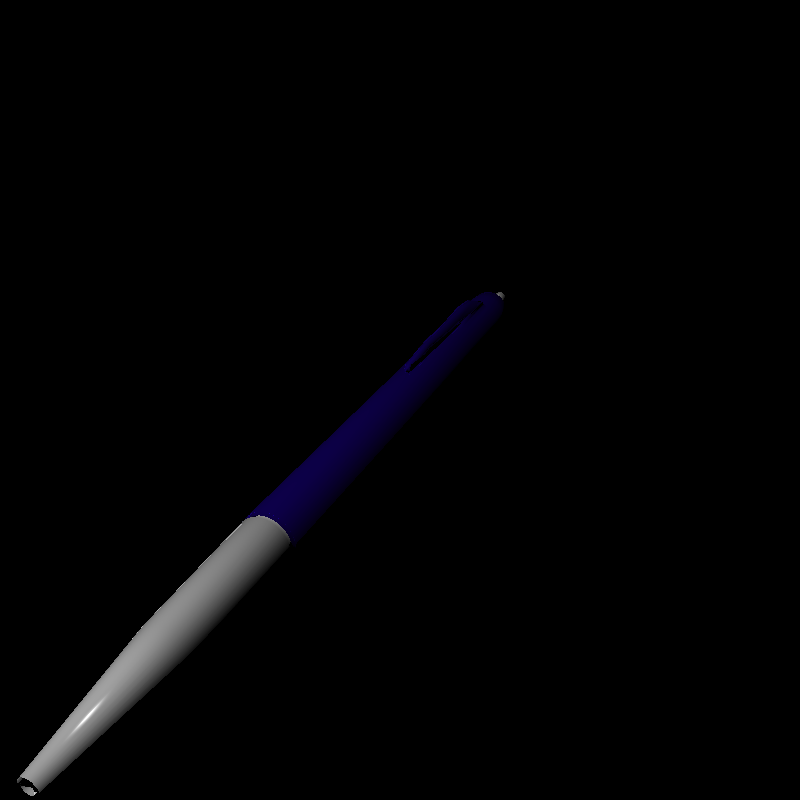
\includegraphics[keepaspectratio,width=8.0cm]{images/interpolate_pen}

Debugging refractions:\\
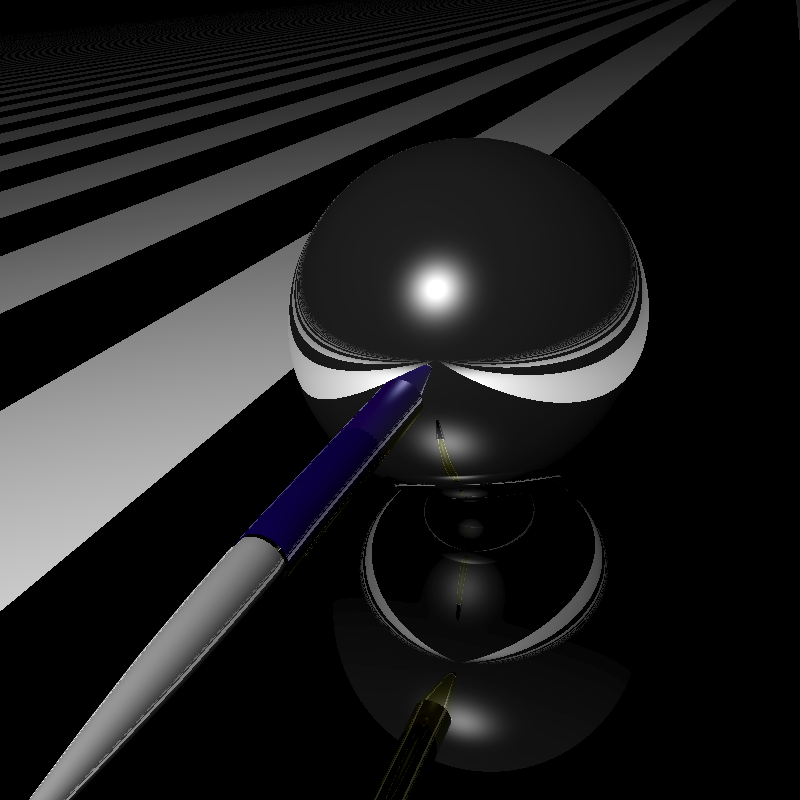
\includegraphics[keepaspectratio,width=8.0cm]{images/master-plane-sphere-pen}\\

\newpage First multi-sampled image:\\
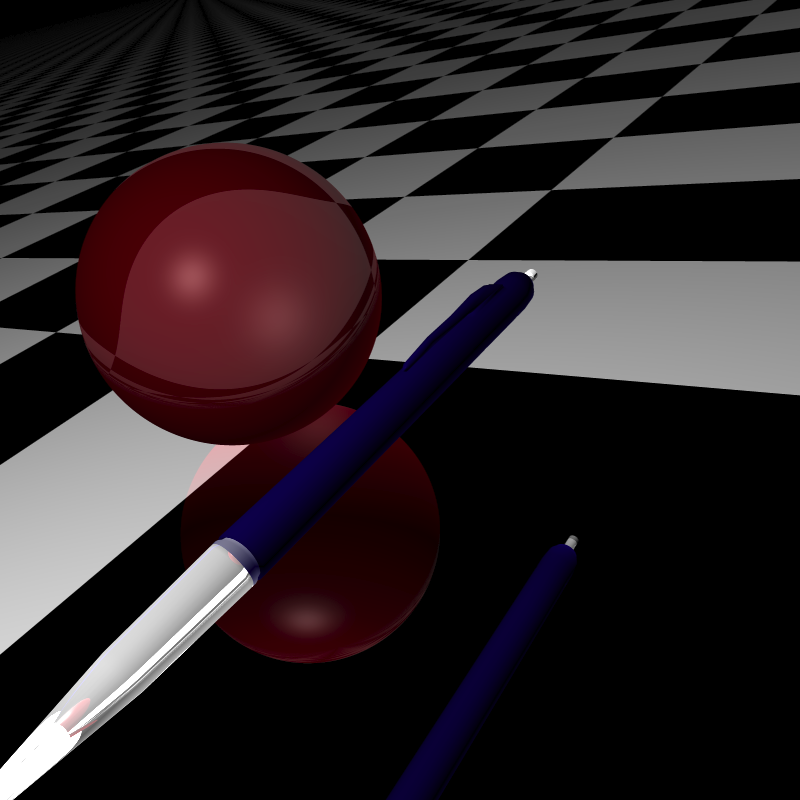
\includegraphics[keepaspectratio,width=8.0cm]{images/multisampling_32x_side.png}\\

Some abstract art (it was a bug, though):\\
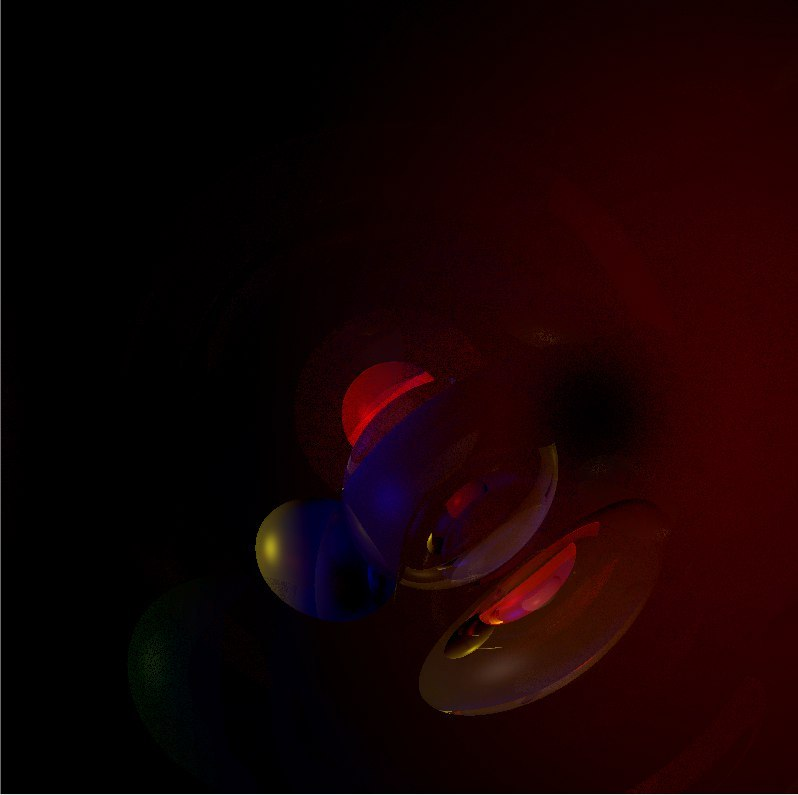
\includegraphics[keepaspectratio,width=8.0cm]{images/abstract_art}\\

\newpage Is this what you get when you're on mushrooms?\\
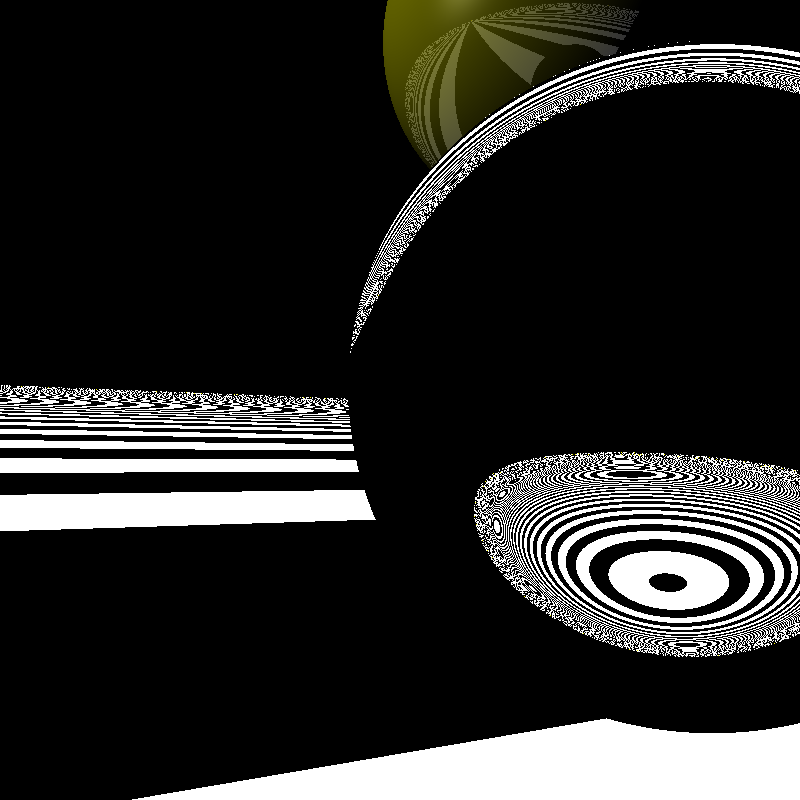
\includegraphics[keepaspectratio,width=8.0cm]{images/tY3lkjt}\\

A first go at textures:\\
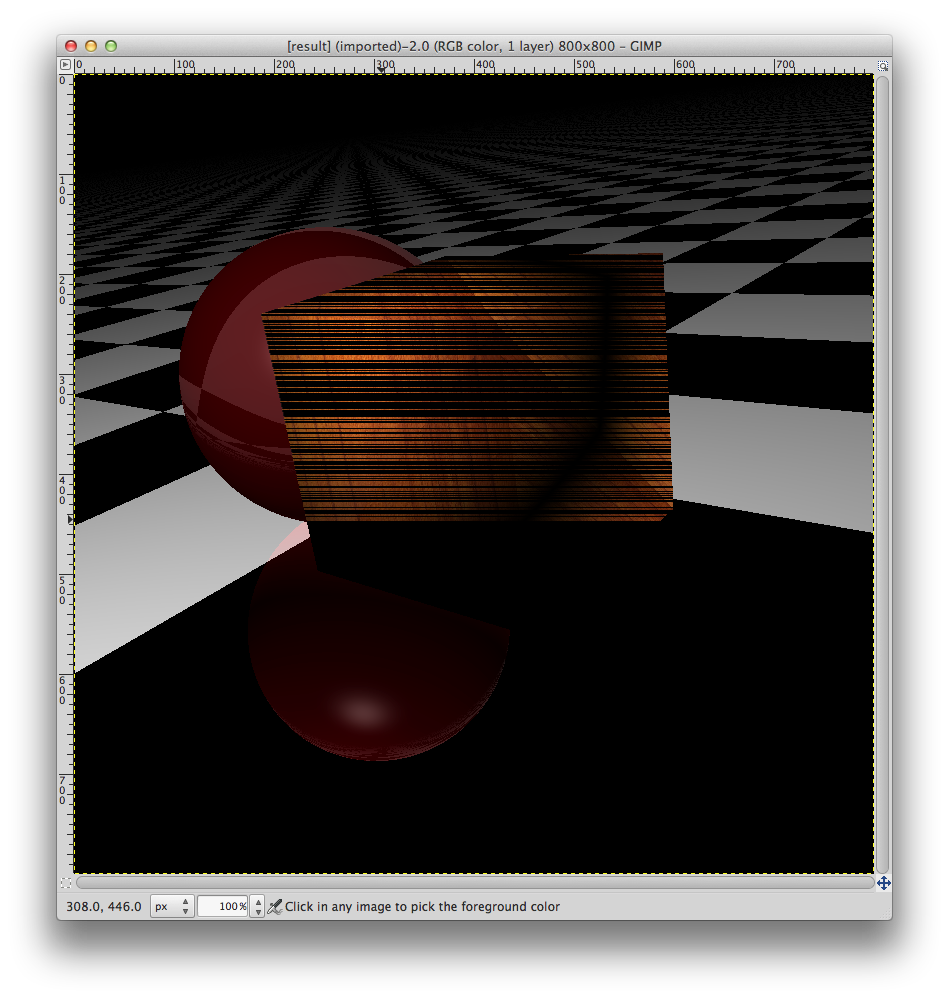
\includegraphics[keepaspectratio,width=8.0cm]{images/texture}\\

\newpage Playing around on tuesday morning:\\
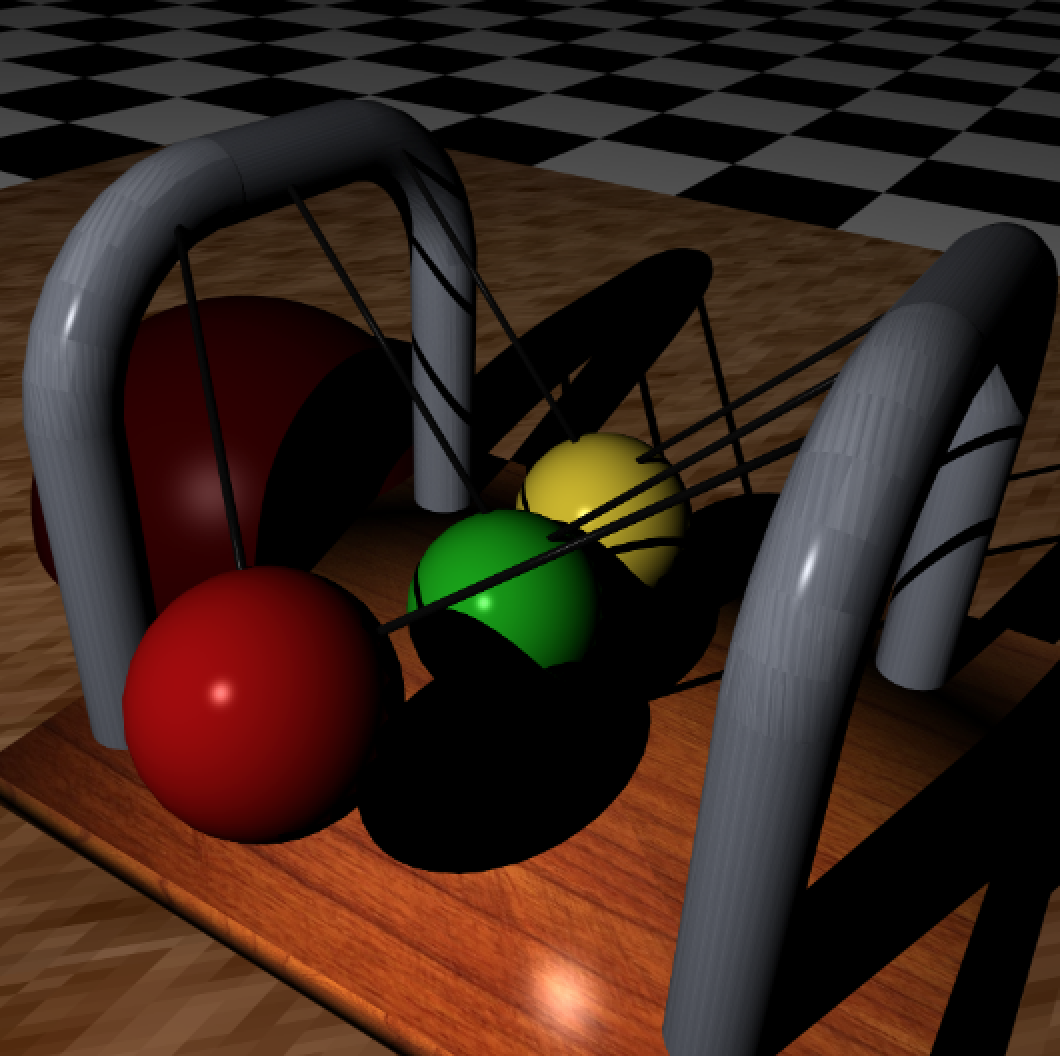
\includegraphics[scale=0.5]{images/playing}\\

Testing multiple shadows:\\
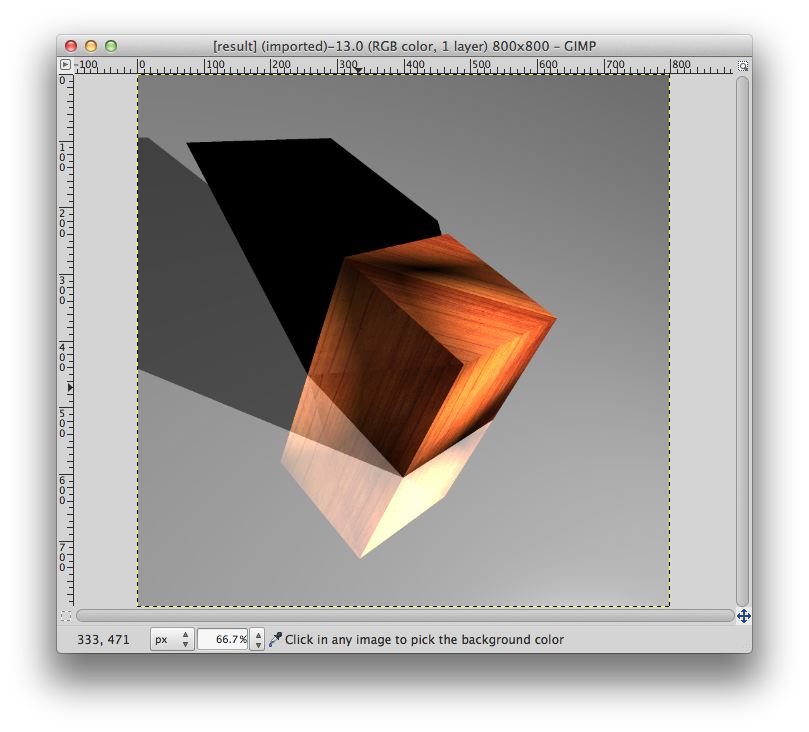
\includegraphics[keepaspectratio,width=8.0cm]{images/mshadow}\\

\end{document}
